\section{Results}

\subsection{Tissue-specific genome-wide gene expression and chromatin accessibility in three tissues}

Gene expression, using RNA-seq, and chromatin accessibility, using ATAC-seq, were measured in lung, liver, and kidney tissues of 47 unique strains in the Collaborative Cross (CC) mouse population. As the function of each tissue is quite distinct, we expected that these data would reflect tissue-specific differences. Principal components analysis (PCA) on each of the gene expression and chromatin accessibility profiles clearly show the clustering of all samples by tissue (\textbf{Figure \ref{fig:pca_plots}}). 

To further validate the quality of these data, we performed pairwise differential expression (DE) and differentially accessible region (DAR) analysis between the three tissues (\textbf{Table \ref{tab:diff_gene}}). We found between 3,564-5,709 DE genes, and 28,048-40,797 DARs across the comparisons. For both expression and chromatin accessibility, liver and kidney tissues were the most similar, and lung and liver were the most distinct, also reflected in the PCA plots. Pathway analyses show between-tissue differences are related mainly to metabolic and immune-related pathways (TO DO: Add GSAA tables (FWER < 0.05) in supplement) and reflects the distinct demands of each tissue. Energy metabolism pathways were more active in liver and kidney and immune-related pathways were more pronounced in lung. We compared the concordance between DE genes and DARs genome-wide and observed that most DE gene promoters do not show significant differences in chromatin accessibility (\textbf{Figure \ref{fig:diff_concordance}}). In cases where there is significantly variable accessibility in the promoter of a DE gene, though, the vast majority agree in direction (i.e. higher expression and greater accessibility). Together, these results support the high quality of the gene expression and chromatin accessibility data.

\begin{figure*}[h]
\renewcommand{\familydefault}{\sfdefault}\normalfont
\centering
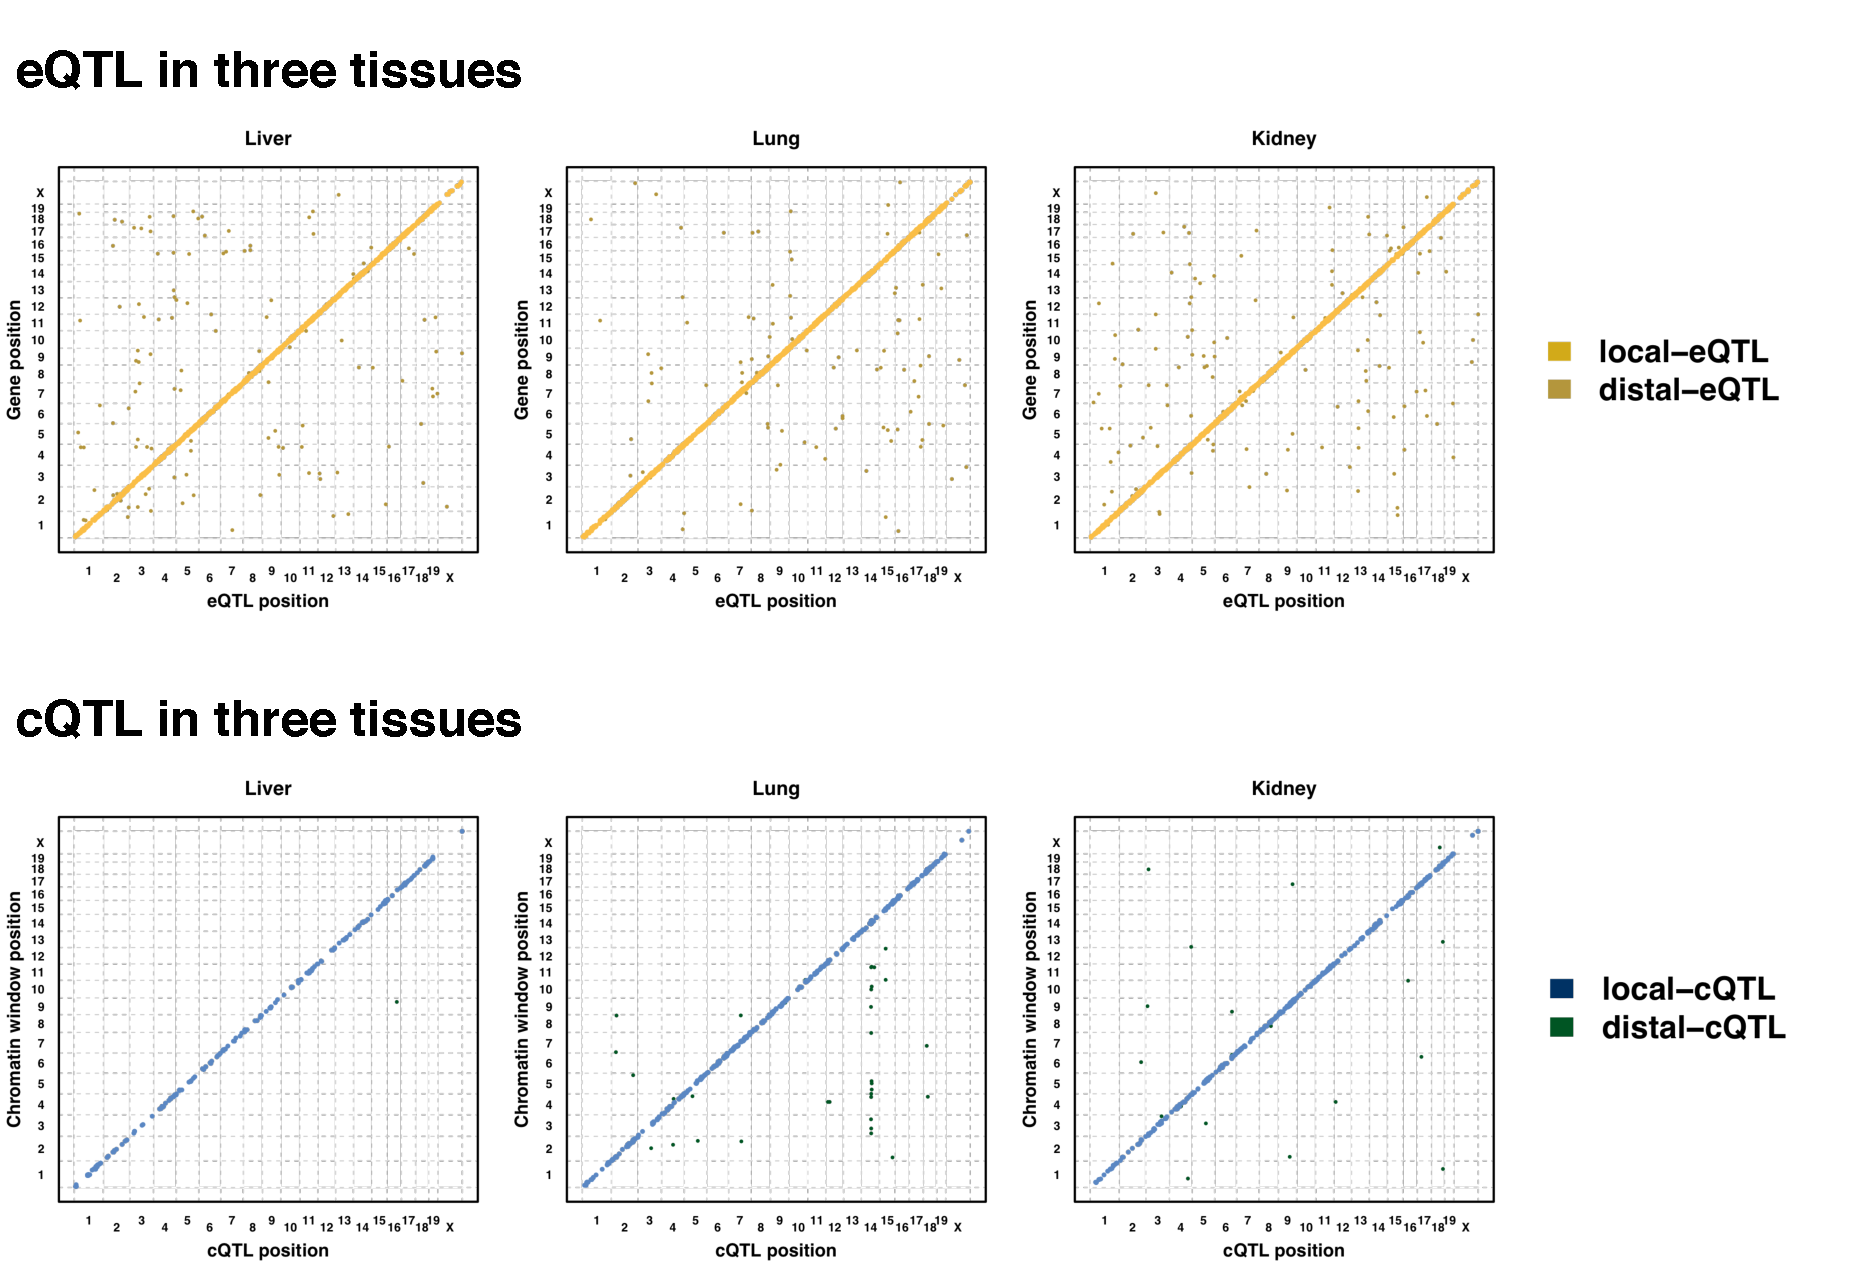
\includegraphics[width=\textwidth, trim={0in 0in 0in 0in}, clip]{figs/qtl_map_main.pdf}
\caption{\textbf{Detected QTL are largely local for both gene expression and chromatin accessibility.} Detected QTL from Method 1 (multi-stage FDR) and Method 3 (genome-wide and chromosome-wide) are included, excluding intra-chromosomal distal-QTL detected through Method 2. The y-axis represents the genomic position of the gene or chromatin site, and the x-axis represents the genomic position of the QTL. Local-QTL appear as dots along the diagonal.
\label{fig:grid_plot}}
\end{figure*}

\subsection{Tissue-specific expression QTL}

To evaluate the impact of genetic variation on gene expression, three approaches to detect eQTL were used, summarized here and described more completely in \textbf{Appendix B}. Method 1 was the most stringent and involved a multi-stage conditional regression procedure paired with an FDR control that allowed for the detection of potentially multiple eQTL per gene and requiring significance at a genome-wide level. Method 2 required FDR-controlled significance at the less stringent chromosome-wide level and only used results from the first stage of the multi-stage analysis, which we refer to as a single-step analysis. Method 3 was also a single-step analysis and employed an even more lenient significance criteria based on the genome-wide and chromosome-wide adjusted FWER p-value. We classified local-eQTL as being within 10 Mb of the transcription start site (TSS) of the gene, and distal-eQTL as being greater than 10 Mb from the TSS on the same chromosome (intra-chromosomal) or on a different chromosome (inter-chromosomal). For Method 2, only local-eQTL and intra-chromosomal distal-eQTL were detected due to our use of chromosome-wide significance criteria. For Method 3, the least stringent method, we only detected local-eQTL.

After filtering lowly expressed genes, a total of 8,401, 11,357, and 10,092 genes were considered for liver, lung, and kidney tissues, respectively. Positions of local-eQTL detected for each tissue using any of the three methods (Method 1, genome-wide q-value < 0.1; Method 2, chromosome-wide q-value < 0.1; Method 3, genome-wide and chromosome-wide FWER p-value < 0.05)  are shown in \textbf{Figure \ref{fig:grid_plot} [top]} (light colored dots), as well as summarized in \textbf{Table \ref{tab:eqtl_mapping}}. We also identified eQTL with Method 1 using a more relaxed significance threshold (q-value < 0.2) in \textbf{Table \ref{tab:eqtl_mapping_lenient}}, which shows that increasing the FDR threshold from 0.1 to 0.2 increases the number of distal-eQTL detected to a greater extent than local-eQTL. Using Method 3 and requiring genome-wide significance, the percentage of tested genes with local-eQTL are 6.3\%, 8.4\%, and 9.5\% for lung, liver, and kidney, respectively (\textbf{Table \ref{tab:eqtl_mapping}}). These percentages increase to 16.6\%, 19.8\%, and 20.8\% when criteria were less stringent with only chromosome-wide significance. 

For each eQTL detected by any of our methods, we estimated the effect size of the eQTL (see \textbf{Tables XX}), defined as the variance component estimate from a random effect fitting of the QTL term (\textbf{Methods}; \textbf{Eq \ref{eq:alternative_model}}), which conservatively constrains the QTL effect in comparison to in the fixed effect genome scan. As expected, Method 1 detects eQTL with large effects (\textbf{Figure \ref{fig:qtl_effect_sizes_by_method}}, red dots). The less stringent Methods 2 and 3 result in greater power to detect local-eQTL with reduced effects (\textbf{Figure \ref{fig:qtl_effect_sizes_by_method}}, gray and blue dots). Distal-eQTL discovered with the multi-stage mapping procedure (Method 1; q-value < 0.1) were detected for $\leq$ 1.6\% of tested genes (\textbf{Table \ref{tab:eqtl_mapping}}; \textbf{Figure \ref{fig:grid_plot} [top]}, dark colored dots), and, consistent with previous studies (\textit{eg} \citealt{Chick2016}), have weaker effects than local-eQTL (\textbf{Figure \ref{fig:qtl_effect_sizes_strict} [top]}). For both Methods 1 and 2, almost three times as many local-eQTL are detected compared to distal-eQTL, likely reflecting these stronger effects. For some distal-eQTL, effect sizes approach zero, potentially resulting from highly influential data points in the fixed effect regression procedure and are thus likely to be false positives. 

To assess whether distance measures to classify intra-chromosomal local- vs distal-eQTL were reasonable, we plotted the statistical association for all intra-chromosomal eQTL from Method 1 (\textbf{Figure \ref{fig:genomewide_dist} [top]}) and the less stringent Method 2 (\textbf{Figure \ref{fig:chrwide_dist} [top]}). In addition to finding that the majority are local-eQTL, we see a drastic reduction in the strength of the statistical association outside of the defined local region. This suggests that intra-chromosomal distal-eQTL are more similar to inter-chromosomal distal-eQTL than local-eQTL, and that our 10Mb boundaries are appropriate. 

Founder allele effects were estimated for all eQTL, using a random effects model to constrain potentially unstable estimates. Consistent with previous studies (\eg \citealt{Aylor2011}), the CAST and PWK alleles tended to have more extreme effects than the classical inbred strains. This pattern was observed for both local and distal eQTL (\textbf{Figure \ref{fig:eqtl_effects_abs}}).

\subsection{Tissue-specific chromatin QTL}

To determine genetic effects on chromatin structure, genomic regions were divided into ~300 base pair windows, and used in chromatin accessibility QTL (cQTL) analysis with the same methods used for eQTL. 11,448, 24,426, and 17,918 chromatin regions were tested in liver, lung, and kidney, respectively. Overall, there were substantially fewer cQTL detected compared to eQTL for all tissues (\textbf{Table \ref{tab:cqtl_mapping}}). Similar to eQTL, cQTL are more likely to be local (66\%-94.1\% for Method 1; 75\%-90\% for Method 2).

Consistent with eQTL, the effect sizes of local-cQTL are on average higher than distal-cQTL (\textbf{Figure \ref{fig:qtl_effect_sizes_strict} [bottom]}), likely contributing to the to the small number of distal-eQTL. cQTL with low effect size are primarily distal-cQTL and may represent false positives. Likewise, most intra-chromosomal cQTL detected using Method 1 or 2 are local-cQTL, and the significance of association is much greater for the local-cQTL  (\textbf{Figure \ref{fig:genomewide_dist} [bottom]} and \textbf{Figure \ref{fig:chrwide_dist} [bottom]}).

The CAST and PWK founder alleles have more extreme than the other strains for local-cQTL, though the pattern is less pronounced, likely due to the reduced number of cQTL (\textbf{Figure \ref{fig:cqtl_effects_abs}}). The numbers of detected distal-cQTL are low, and no clear trends obvious.

\section{QTL detected in multiple tissues}

For a given trait, QTL from different tissues were paired based on co-localizing to approximately the same genomic region. For local-QTL, both had to be within the local window, defined at 10 Mb around the gene TSS, resulting in a maximum distance of 20 Mb between QTL. For distal-eQTL, both had to be within 10 Mb of each other. 

For local-eQTL, 761 pairs were found for liver and lung, 1,206 for liver and kidney, and 1,025 for lung and kidney. In distal-eQTL, 61 pairs were made in liver and lung, 120 in liver and kidney, and 59 in lung and kidney. For cQTL, the vast majority of pairs were local, with 55 between liver and lung, 56 between liver and kidney, and 142 between lung and kidney. Only 4 distal-cQTL pairs were observed, all being shared between lung and kidney. The effect sizes of paired QTL vary across tissues, though they were significantly correlated, shown in \textbf{Figure \ref{fig:qtl_effect_size_comparison}}.

The correlation between the founder allele effects for pairs of QTL were calculated. Highly correlated QTL pairs tended to be highly proximal to each other (\textbf{Figure \ref{fig:qtl_cor_by_distance_comparison}}), suggesting that the underlying causal variants are the same or related. The null hypothesis of uncorrelated QTL effects was tested through a t-test, and positively correlated pairs of QTL identified, significant at FDR $\leq 0.1$ for each pairwise comparison of tissues (\textbf{Figure \ref{fig:qtl_pair_histograms}}). 345, 623, and 498 local-eQTL pairs were positively correlated for liver versus lung, liver versus kidney, and lung versus kidney, respectively. For distal-eQTL, 21, 34, and 16 positively correlated pairs were found for the same tissue comparisons. For local-cQTL, 47, 48, and 118 positively correlated pairs were identified. With only four pairs of distal-cQTL between lung and kidney, there were not a sufficient number of tests to use with an FDR procedure. However, three of the four pairs had correlations greater than 0.5. Negatively correlated QTL pairs were identified, but based on the FDR control for multiple testing, none were significantly negatively correlated.

\begin{figure*}[h]
\renewcommand{\familydefault}{\sfdefault}\normalfont
\centering
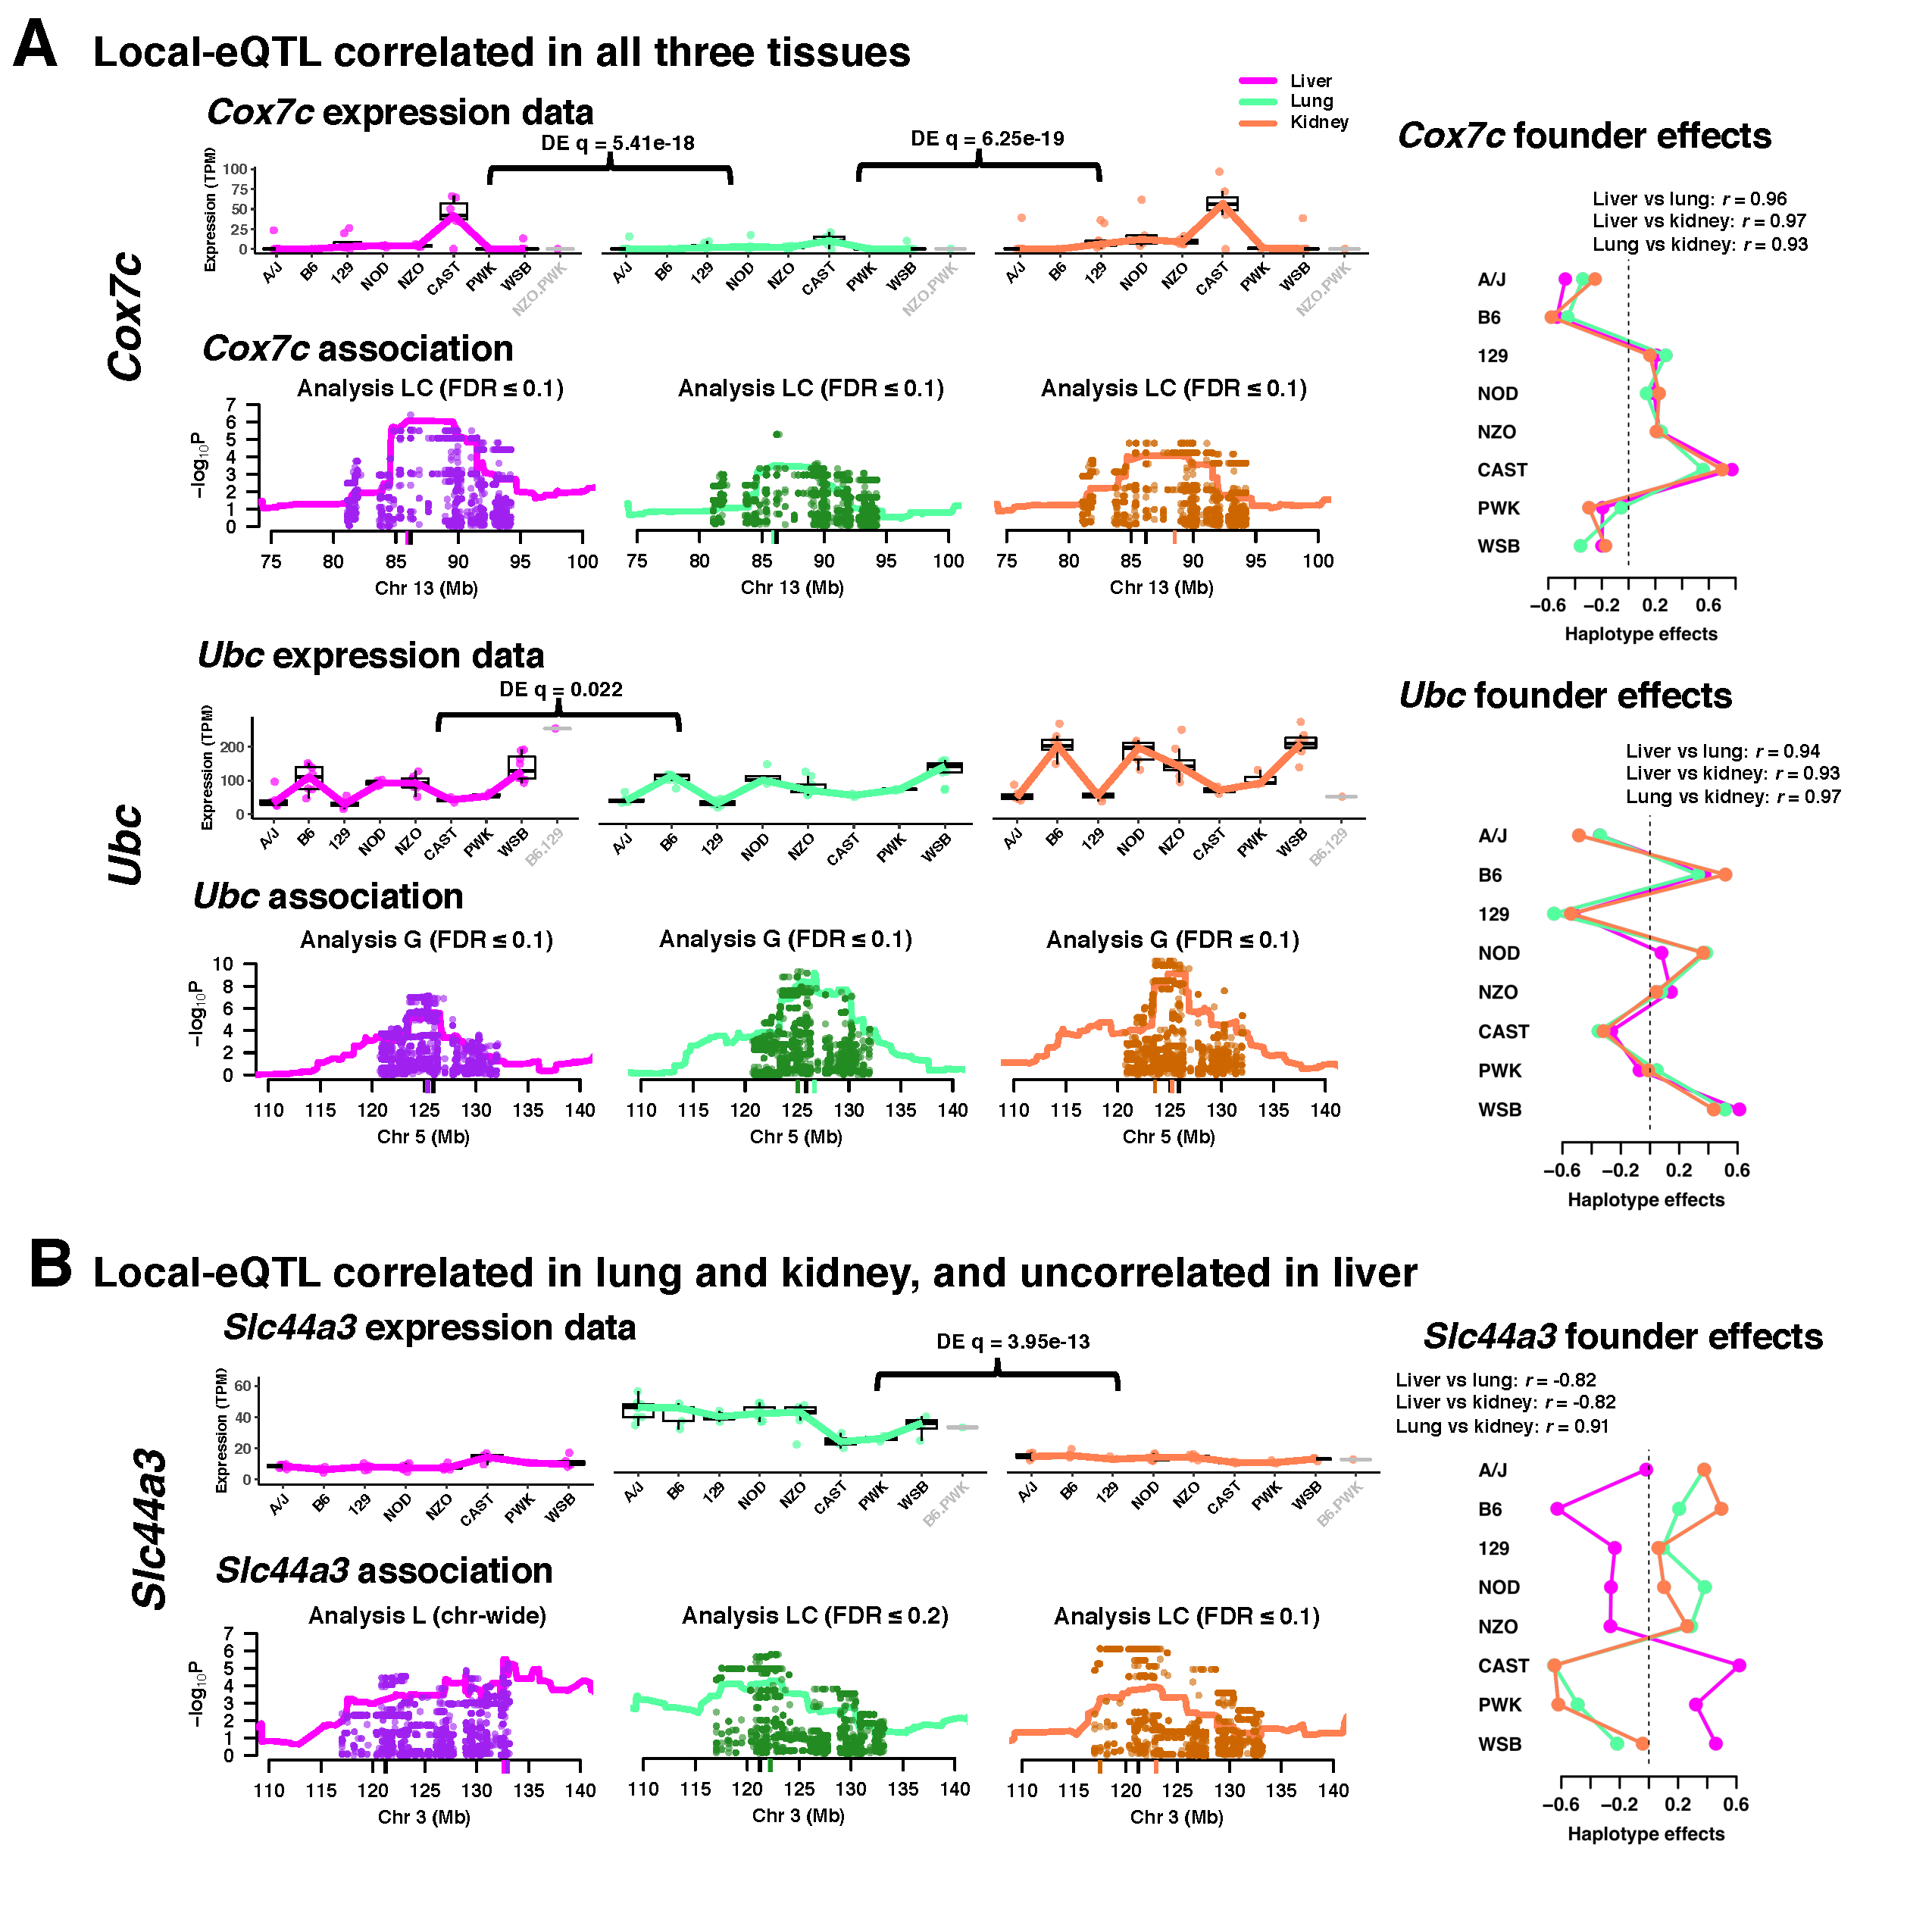
\includegraphics[width=0.8\textwidth, trim={0in 0.5in 0in 0in}, clip]{figs/correlated_local_eqtl.pdf}
\caption{\textbf{Examples of genes with local-eQTL observed in all three tissues.}\label{fig:correlated_local_eqtl}}
\end{figure*}

\subsection{Genes with correlated local-eQTL: \textit{Cox7c} and \textit{Ubc}}

Correlated QTL effects suggest that the detected QTL stem from the same or related causal variants, active within both tissues, and is largely seen in both eQTL and cQTL, local and distal. Local-eQTL with strong statistical provide some clear examples in cytochrome c oxidase subunit 7C (\textit{Cox7c}) and ubiquitin C (\textit{Ubc}).

\textit{Cox7c} and \textit{Ubc} posses local-eQTL with highly correlated effects in all three tissues (\textbf{Figure \ref{fig:correlated_local_eqtl}}). Based on the expression data and founder effects, the \textit{Cox7c} local-eQTL has a high CAST allele, intermediate alleles from 129, NOD, and NZO, and ow alleles in A/J, B6, PWK, and WSB. \textit{Ubc} has a different pattern of founder alleles, with high alleles attributed to B6, NOD, NZO, and WSB. Notably, these founder effects are consistent across tissues with distinctly different overall patterns of expression for \textit{Cox7c} and \textit{Ubc}. The expression of \textit{Cox7c} is significantly higher in liver compared to both lung ($q = 5.41e-18$) and kidney ($q = 6.25e-19$). For \textit{Ubc}, liver and lung had slight differential expression ($q = 0.022$). The haplotype and variant associations in the local region match closely for all tissues for both \textit{Cox7c} and \textit{Ubc}. Though all the \textit{Ubc} local-eQTL were detected with the most stringent Method 1, the \textit{Cox7c} local-eQTL were detected with the more lenient Method 2.

\subsection{Genes with uncorrelated local-eQTL: \textit{Slc44a3} and \textit{Pik3c2g}}

Uncorrelated QTL potentially represent multiple tissue-specific QTL: genetic variants that influence gene expression or chromatin accessibility in a specific tissue. Solute carrier family 44, member 3 (\textit{Slc44a3}) is an interesting example, having correlated local-eQTL effects in lung and kidney, and unique effects in liver. Notably, the effects in liver are anti-correlated with the effects in lung and kidney, suggesting the liver eQTL could be transgressive \citep{Rieseberg1999} to the eQTL in lung and kidney, whereby the effects of the founder alleles are reversed. For \textit{Slc44a3}, CAST, PWK, and WSB have high alleles for the liver eQTL, but low alleles in lung and kidney. The haplotype and variant association for \textit{Slc44a3} look more similar for lung and kidney, with the liver eQTL being more distal to the gene TSS, near the 10 Mb boundary used to categorize QTL as local or intra-chromosomal distal-QTL. Overall, the expression data, estimated effects, and patterns of association are consistent with lung and kidney sharing a causal local-eQTL, and liver possessing a unique one. The lung eQTL was detected with the highly lenient Method 2 (FDR $\leq$ 0.2) and the kidney eQTL with the less lenient Method 2 (FDR $\leq$ 0.1). The liver eQTL was detected with the lenient Method 3 (chromosome-wide). 

Phosphatidylinositol-4-phosphate 3-kinase catalytic subunit type 2 gamma (\textit{Pik3c2g}), a gene of interest for diabetes-related traits \citep{Braccini2015}, has local-eQTL in each of the three tissues that are not correlated with each other. The overall magnitude of expression varies across the three tissues, at statistically significant levels for liver versus lung ($q = \num{3.12e-13}$) and lung versus kidney ($q = \num{3.55e-6}$). The presence of tissue-specific local-eQTL is further supported by the \textit{Mus musculus} lineages in the genomic region local to \textit{Pik3c2g}. The founder strains of the CC all possess contributions from three subspecies of \textit{M. musculus}: \textit{domesticus} (\textit{dom}), \textit{castaneus}, (\textit{cast}), and \textit{musculus} (\textit{mus}) \citep{Yang2011}. \cite{Crowley2015} found that allele-specific gene expression in mice descended from the CC founders often followed patterns that matched the subspecies inheritance at the gene regions.

\begin{figure*}[h]
\renewcommand{\familydefault}{\sfdefault}\normalfont
\centering
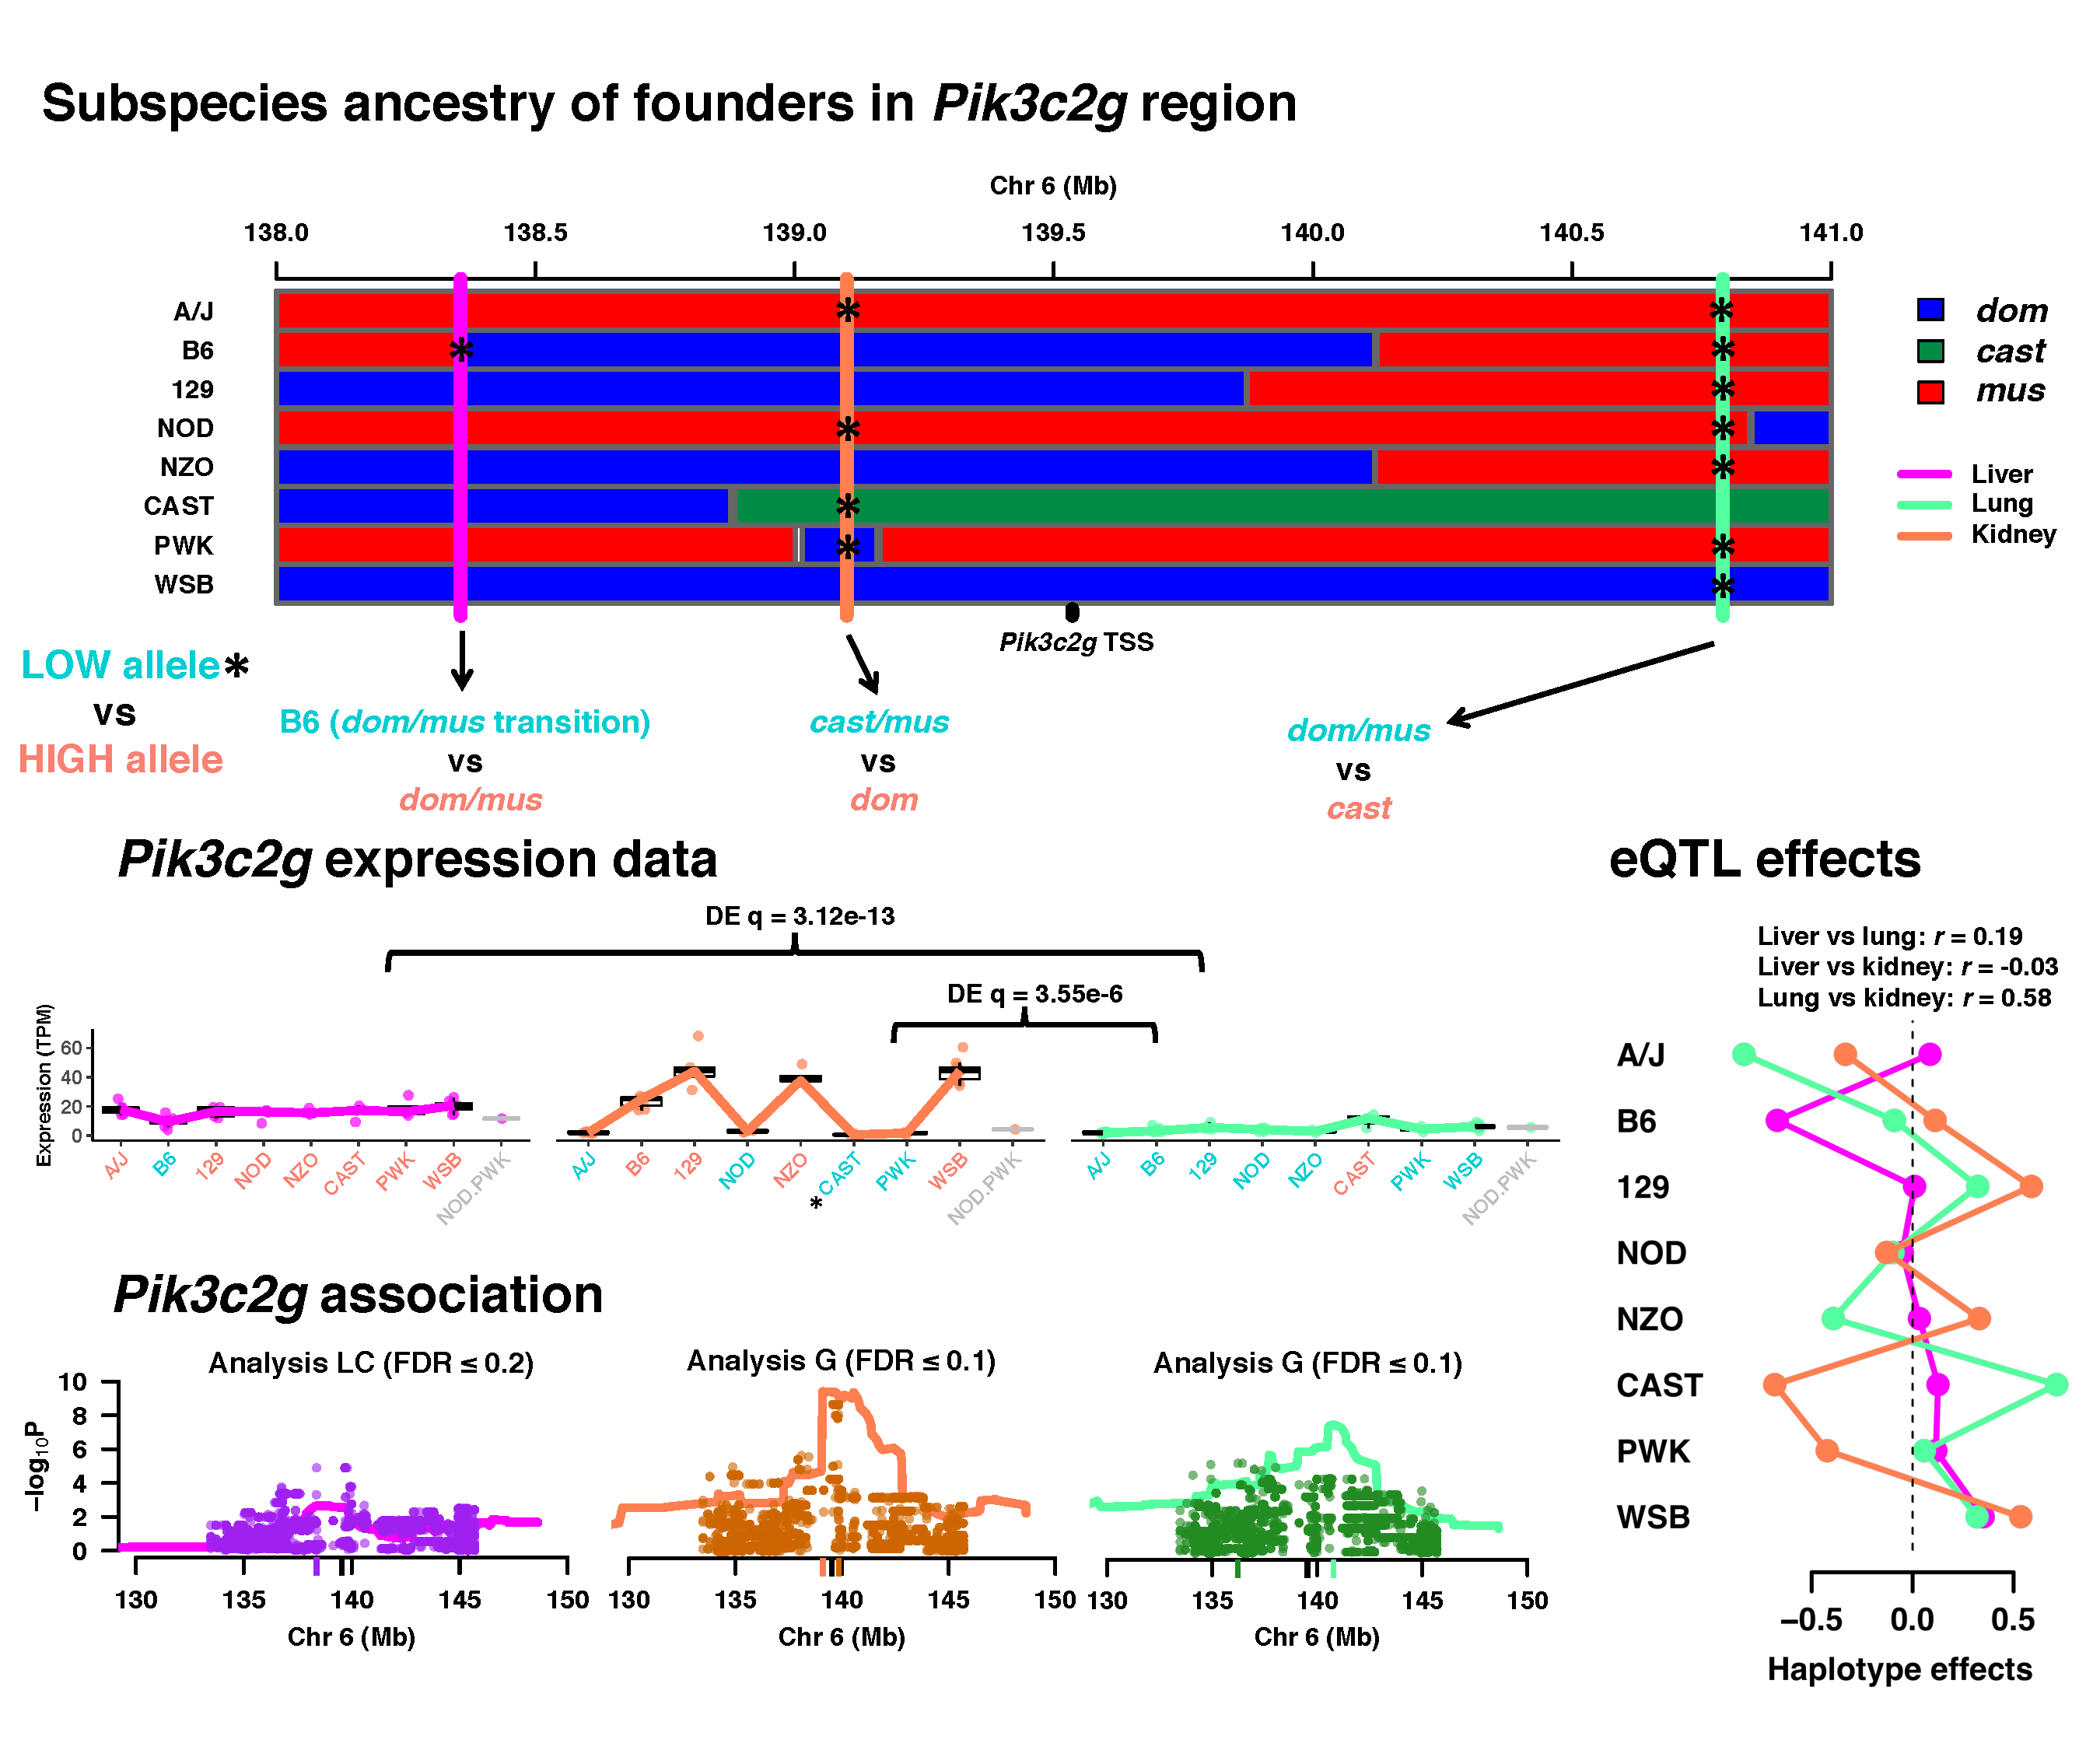
\includegraphics[width=0.8\textwidth, trim={0in 0.5in 0in 0in}, clip]{figs/pik3c2g_example.pdf}
\caption{\textbf{\textit{Pik3c2g} possesses tissue-specific local-eQTL.}\label{fig:pik3c2g}}
\end{figure*}

The lung eQTL, detected with high significance through Method 1, has a high effect from the CAST founder, which possesses the \textit{cast} subspecies lineage at the locus, consistent with a \textit{cast} versus \textit{dom}/\textit{mus} allelic series. The kidney eQTL, also highly statistically significant (Method 1), is closest to the \textit{Pik3c2g} TSS. Mice with contributions from B6, 129, NZO, and WSB have high expression whereas nearly no expression in mice with contributions from A/J, NOD, CAST, and PWK, mostly consistent with a \textit{dom} versus \textit{cast}/\textit{mus} allelic series. The PWK founder has a small \textit{dom} haplotype block at the QTL peak in a broader region that is largely \textit{mus}. The expression data are highly consistent with PWK having the \textit{mus} allele, suggesting that the causal variant is located in the nearby regions, which is supported by the variant association. Notably, the B6 allele appears intermediate to the other founders that possess \textit{dom} inheritance, representing a potentially multi-allelic QTL that haplotype association can better identify in comparison to bi-allelic variant association. The liver eQTL, identified with Method 2 and a very lenient FDR $\leq 0.2$, was characterized by a low B6 allele. The B6 founder does not have a unique subspecies lineage at the locus, but instead possesses a recombination event between \textit{dom} and \textit{mus}, potentially disrupting the local regulation specific to each subspecies lineage and explaining the low effect.

\subsection{Genes with distal-QTL observed across tissues: \textit{Akr1e1}, \textit{Per2}, and \textit{Rnf13}}

Founder allele effects that correlate across tissues can provide stronger confirmation of distal-QTL. Though fewer distal-QTL were significantly correlated across tissues in comparison to local-QTL (71 to 1,466 for eQTL and 2 to 213), potentially reflecting the reduced power to detect distal-QTL in this study, a number of genes were identified with unique patterns of distal-eQTL over the tissues, shown in \textbf{Figure \ref{fig:correlated_distal_eqtl}}.

Located on chromosome 13, Aldo-keto reductase family 1, member E1 (\textit{Akr1e1}) had no local-eQTL detected in any of the tissues. Distal-eQTL were detected in all tissues that localize to the same distal region of chromosome 4. The founder allele effects of the distal-eQTL are all highly correlated, with A/J, B6, 129, and CAST representing highly expressing alleles. The overall magnitude of expression varies significantly across the tissues, with liver and kidney having significantly higher expression than lung ($q = \num{1.63e-19}$ and $q = \num{4.40e-34}$, respectively). The distal-eQTL for \textit{Akr1e1} will be discussed further with the topic of mediation.

As with local-QTL, correlated distal-eQTL can provide strong evidence that marginally significant QTL are valid. Period circadian clock 2 (\textit{Per2}) possesses intra-chromosomal distal-eQTL that are detected in all three tissues and approximately 100 Mb away from the gene TSS, detected with the highly lenient Method 2 (FDR $\leq$ 0.2). However, the founder allele effects are significantly correlated among the tissues, characterized by high NOD and PWK alleles. Collectively, these findings provide strong validation for the distal-eQTL, which would commonly not be detected.

QTL analysis in multiple tissues also allows for the detection of tissue-specific distal-QTL. Ring finger protein 13 (\textit{Rnf13}) is an interesting example. Across all the tissues, \textit{Rnf13} was lowly expressed. Nevertheless, a strong local-eQTL was detected in liver. Using the multi-stage conditional regression approach, conditioning on the local-eQTL resulted in a distal-eQTL on chromosome 12 being detected, which was only suggestive in the first scan. Comparing the residuals after regressing out the local-eQTL and founder allele effects suggests that mice with B6 contributions at the distal locus had higher \textit{Rnf13} expression. In lung tissue, a distal-eQTL was detected on the X chromosome with a different founder allele pattern, notably high A/J, B6, and PWK alleles, and low NOD and NZO alleles. These examples demonstrate that analyzing multiple tissues can provide greater evidence of distal-QTL, as well as potentially identify tissue-specific genetic regulation.

\begin{figure*}[h]
\renewcommand{\familydefault}{\sfdefault}\normalfont
\centering
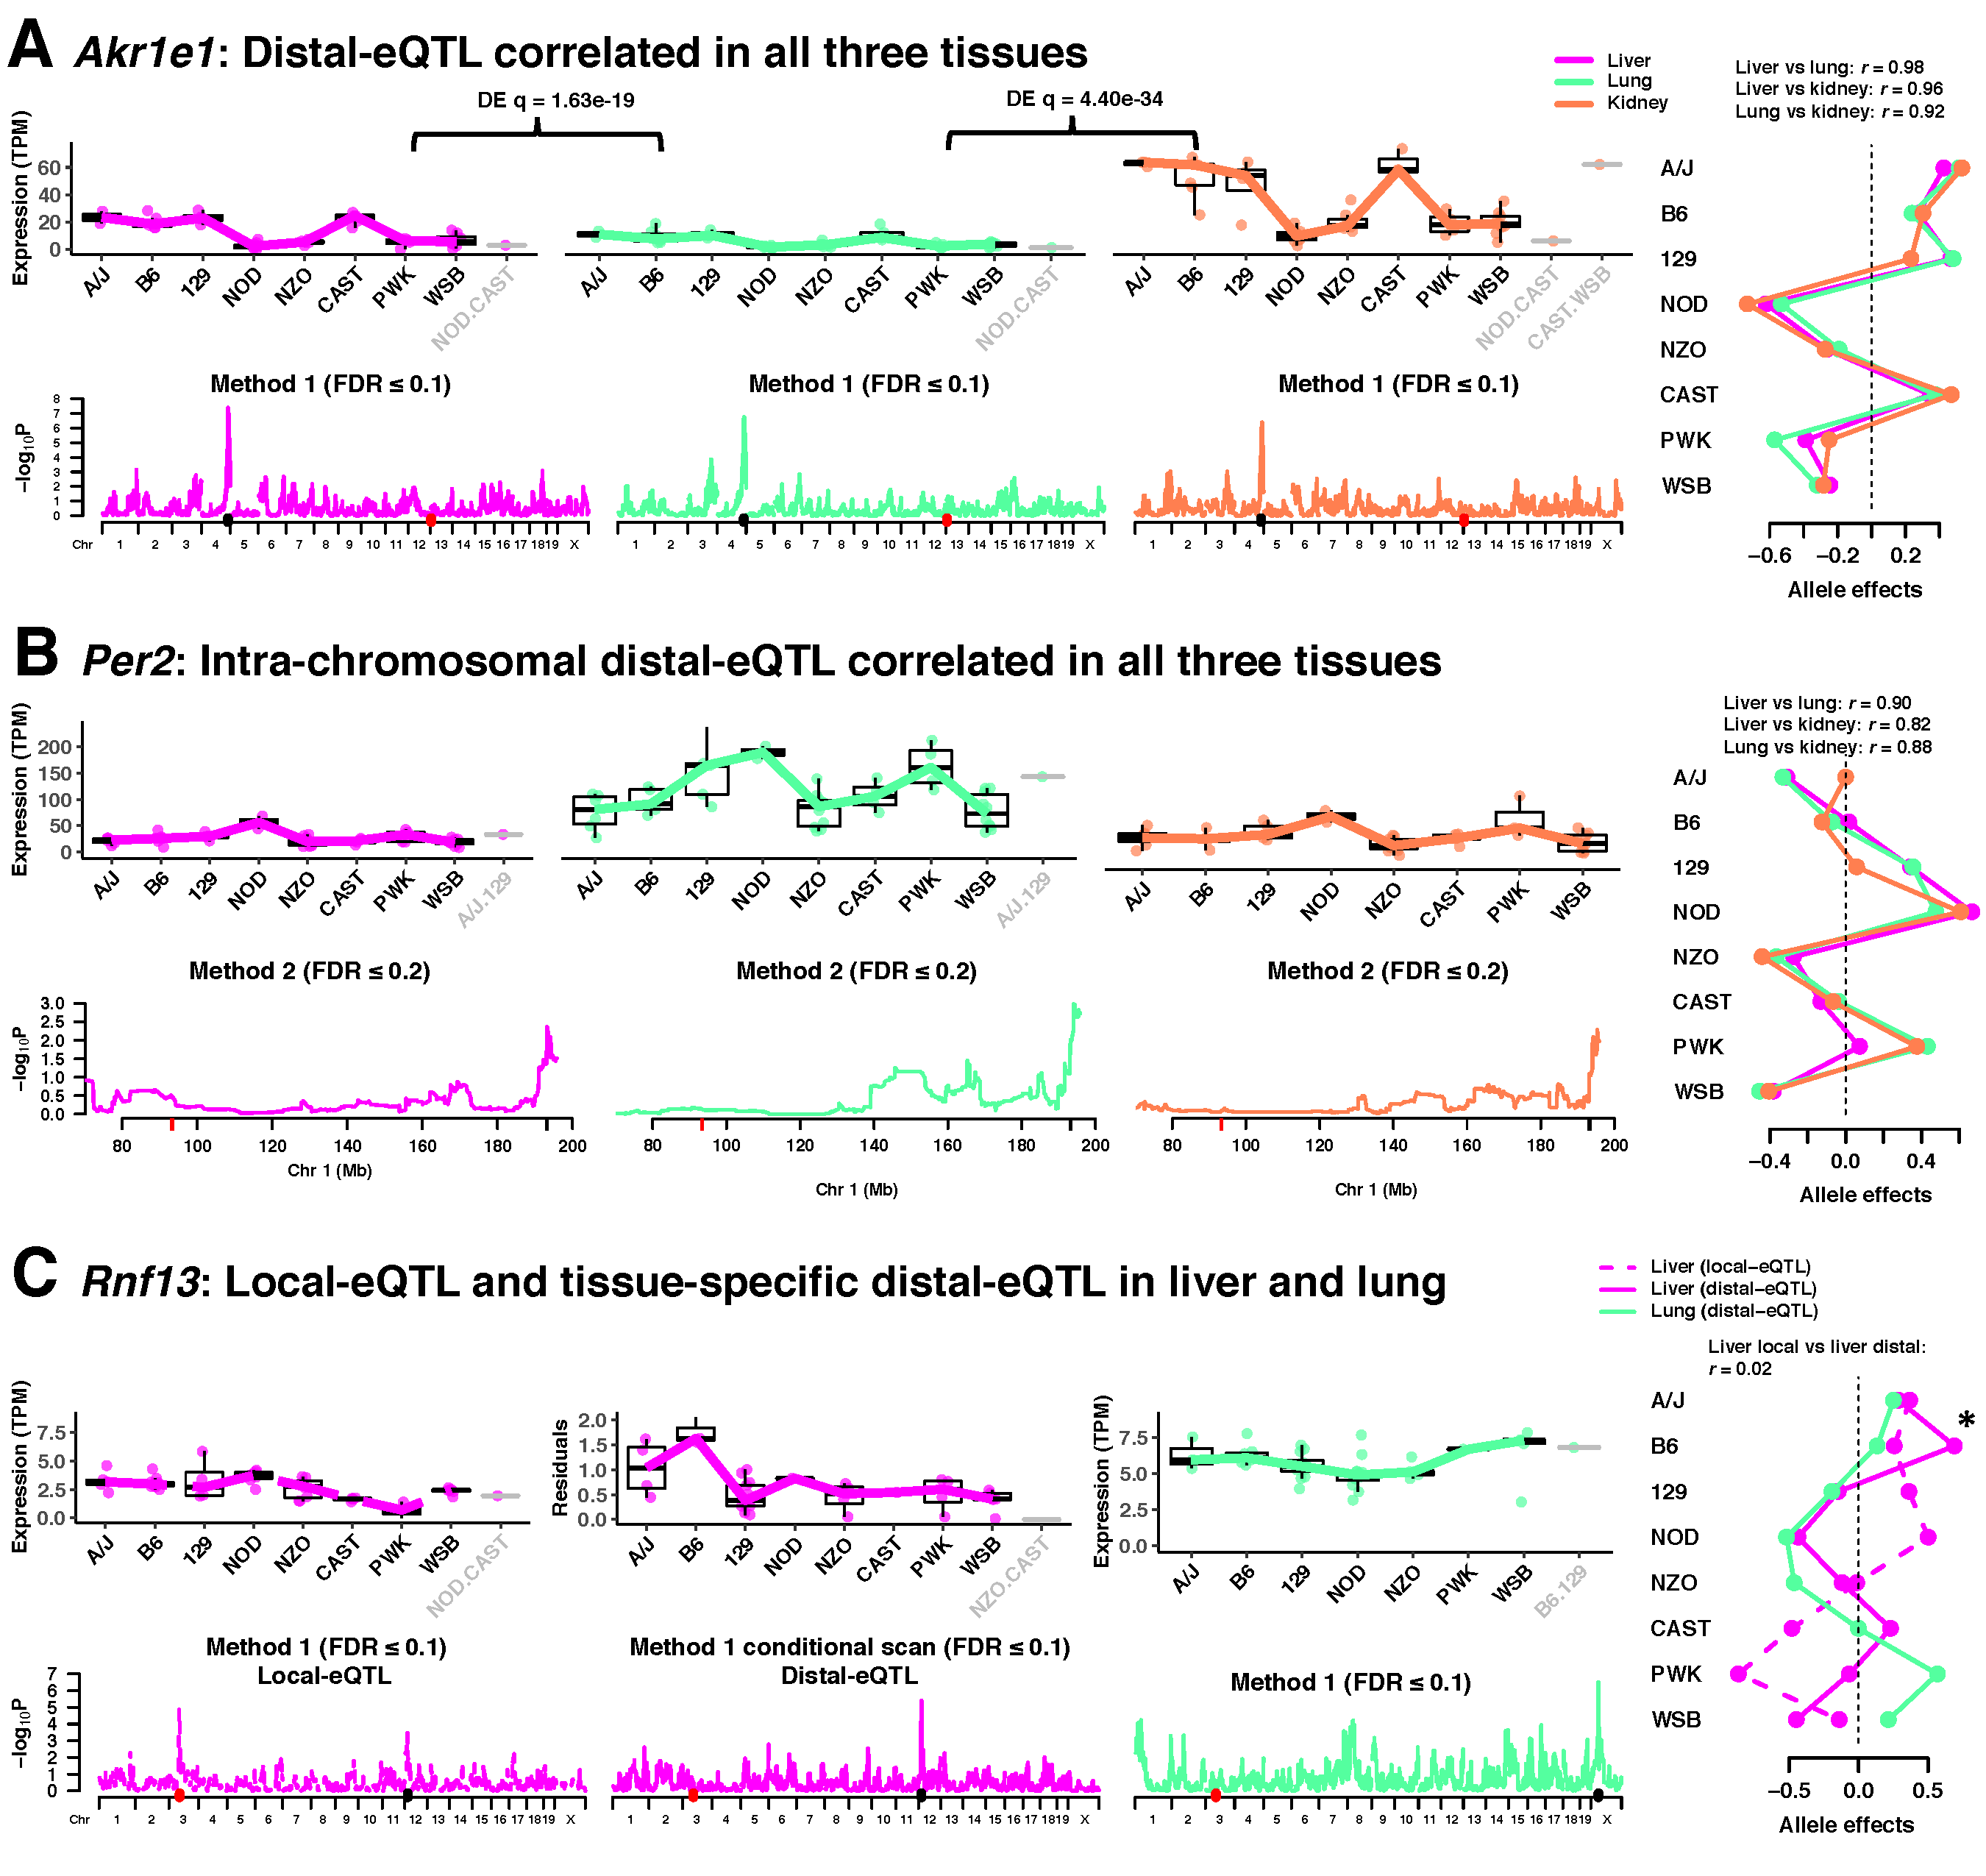
\includegraphics[width=0.8\textwidth, trim={0in 0in 0in 0in}, clip]{figs/correlated_distal_eqtl.pdf}
\caption{\textbf{Examples of genes with distal-eQTL effect patterns across tissues.}\label{fig:correlated_distal_eqtl}}
\end{figure*}

\section{Mediation}

Measurement of gene expression and chromatin accessibility data in the same mice and tissues enables the use of mediation analysis to elucidate the relationships between genotype, chromatin accessibility, and gene expressions; we assess evidence for two mediation models of eQTL effects (\textbf{Figure \ref{fig:graph}}). First, proximal chromatin state as a mediator of the effect of local-eQTL on gene expression. Second, expression levels of proximal genes as a mediator of distal-eQTL effect. For the first mediation model, we used an approach adapted from \cite{Chick2016} to detect mediation through chromatin accessibility of local-eQTL detected through Method 3 (genome-wide and chromosome-wide). For the second mediation model, we use an approach similar to \cite{Keller2018} to assess statistically significant mediation of distal-eQTL detected by Method 1; see \textbf{Appendix C} for greater detail.  

\begin{figure*}[h]
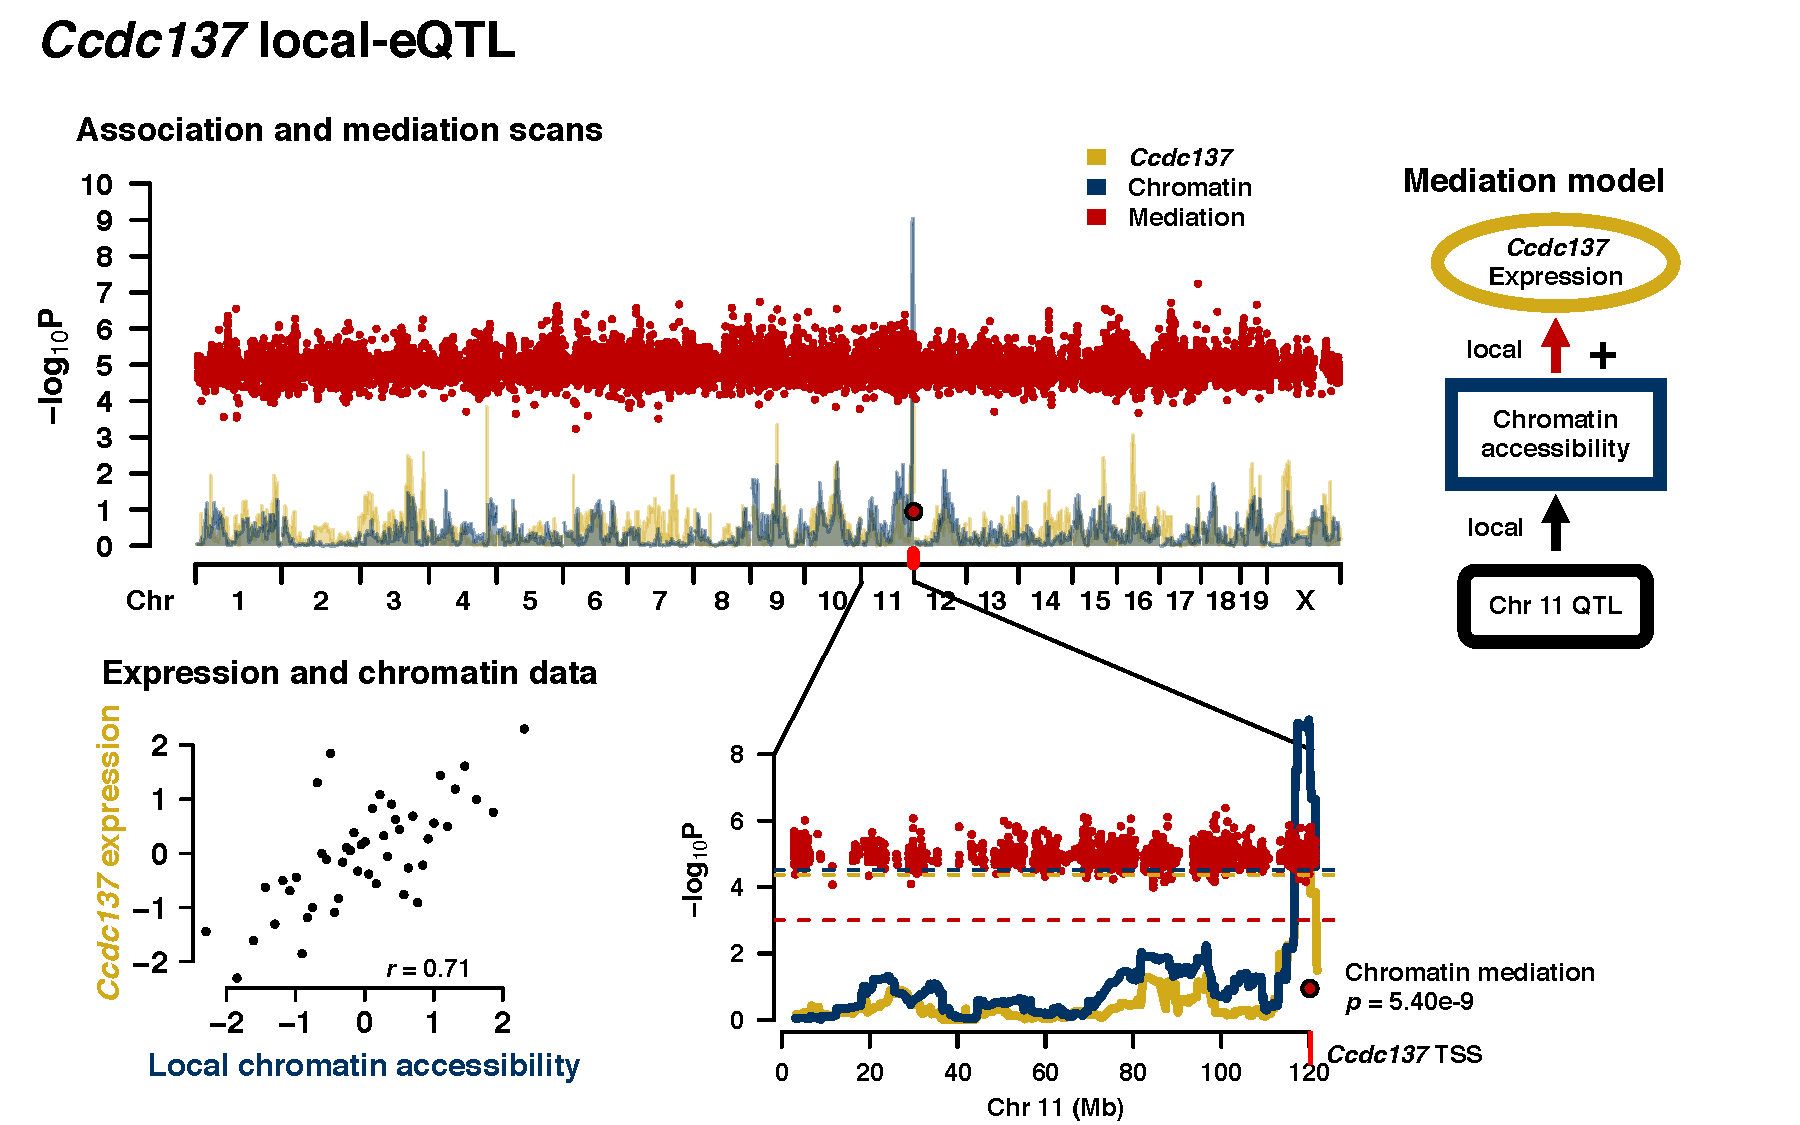
\includegraphics[width=\textwidth, trim={0in 0in 0in 0in}, clip]{figs/ccdc137_mediation.pdf}
\caption{\textbf{QTL and mediation scans.} Genome scans for \textit{Ccdc137} expression (yellow), chromatin accessibility (blue), and chromatin mediation (red), a gene located on chromosome 11, in lung tissue of 47 CC strains. There are strong co-localizing local-eQTL and local-cQTL near the TSS of \textit{Ccdc137} (red tick). The steep logP drop for a single chromatin site outcome in the mediation scan at the co-localizing QTL strongly suggests chromatin mediation of \textit{Ccdc137} expression is present. The QTL and mediation signals are significant at both genome-wide levels (A) and at chromosome-wide levels (B). \label{fig:ccdc137_mediation}}
\end{figure*}

\subsection{Mediation of local-eQTL effects through proximal chromatin accessibility}

We found 30-68 local-eQTL showed evidence of mediation through proximal chromatin accessibility at genome-wide significance, and 70-181 at chromosome-wide significance (\textbf{Table \ref{tab:mediation}}). The coiled-coil domain containing 137 gene (\textit{Ccdc137}) is a strong example of mediation through local chromatin accessibility. \textbf{Figure \ref{fig:ccdc137_mediation}} includes the genome scans that identify local-QTL for \textit{Ccdc137} expression (eQTL) and a proximal chromatin accessibility window (cQTL). The red tick marks the TSS for \textit{Ccdc137}, which is highly proximal where both the eQTL and cQTL are mapping. The red dots represent the significance of the eQTL after conditioning on each chromatin region as a mediator. A large drop in eQTL significance at the location of the cQTL represents a strong mediation signal. A closer inspection of the region shows that the significance of the eQTL and cQTL are similar but notably stronger for chromatin, as expected by the proposed mediator model. 

Highly proximal eQTL and cQTL, \textit{i.e.} co-localization, is not sufficient for mediation, shown in \textbf{Figure \ref{fig:colocalization}}. For both \textit{Hdhd3} in liver (\textbf{Figure \ref{fig:colocalization} [left]}) and the acyl-Coenzyme A binding domain containing 4 gene (\textit{Acbd4}) in kidney (\textbf{Figure \ref{fig:colocalization} [right]}), there is a local-eQTL with a co-localizing cQTL. Comparing the statistical associations at the genomic locations of the eQTL and cQTL as well as the founder haplotype effects for both the eQTL and cQTL, the correspondence in both is greater for \textit{Hdhd3} compared to \textit{Acbd4}. As with \textit{Ccdc137}, a strong mediation signal is detected for \textit{Hdhd3}, indicated by the decrease in the eQTL association when conditioning on the chromatin state. Mediation is not detected for \textit{Abcd4}, which is consistent with the genetic regulation of both gene and chromatin site not stemming from the same causal origin.

\subsection{Mediation of distal-eQTL effects through proximal gene expression}

A related mediation model was used to identify genome-wide significant distal-eQTL that are mediated through the expression of proximal genes, as might be expected for a transcription factor with its own local-eQTL (\textbf{Figure \ref{fig:graph} B}). Eight genes were identified with mediation of distal-eQTL (\textbf{Table \ref{tab:exmediation}}), including cyclin Y-like 1 (\textit{Ccnyl1}), which is mediated in lung by the expression of a zinc finger protein, which characteristically have DNA-binding functionality and often act as transcription factors. The mediation of \textit{Ccnyl1} expression is illustrated in \textbf{Figure \ref{fig:ccnyl1_exmediation}}. The founder haplotype effects at the distal-eQTL of \textit{Ccnyl1} are highly correlated with the local-eQTL effects for zinc finger protein 979 (\textit{Zfp979}), though with a reduction in overall strength, in accordance with the proposed mediation model.

\subsection{Proposed model of the genetic regulation of \textit{Akr1e1}}

Another gene with a strong mediation signal through proximal gene expression is \textit{Akr1e1}, which we described earlier as having strong distal-eQTL observed in all three tissues with correlated founder effects. Zing finger protein 985 (\textit{Zfp985}) was identified as a strong mediator that his highly proximal to the distal eQTL on chromosome 4; the \textit{Zfp985} TSS is located at 147.6 Mb compared to the distal-eQTL coordinates of 142.5 Mb, 143.2 Mb, and 148.6 Mb in liver, lung, and kidney, respectively (\textbf{Figure \ref{fig:akr1e1_exmediation}}).

The presence of distal genetic regulation for \textit{Akr1e1} was previously described by \cite{HamiltonWilliams2013}. The distal-eQTL we detect are highly proximal to the \textit{Idd9.2} region \citep{HamiltonWilliams2010}, which approximately spans 145.5-148.57 Mb of chromosome 4. \cite{HamiltonWilliams2013} fine-mapped the \textit{Idd9.2} region using NOD mice congenic with C57BL/10 (B10) introgressions. Consistent with the previous studies, CC strains with NOD inheritance at the distal-eQTL have low expression of \textit{Akr1e1}. Genetic variation from B10 is not present in the CC, but the B6 founder is a closely related substrain and has high expression of \textit{Akr1e1}, which is consistent with B10. The other CC founders allele effects fall into approximately high and low groups, with NZO, PWK, and WSB joining NOD in a low \textit{Akr1e1} expressing group, and A/J, 129, and CAST with B6 as a high expressing group (\textbf{Figure \ref{fig:correlated_distal_eqtl}A}). 

All eQTL, cQTL, and mediation results for all three tissues are represented in \textbf{Figure \ref{fig:circos_plot}}. Notably, distal eQTL and cQTL are not evenly distributed across the genome. In particular, there is a high concentration of chromatin mediation detected along chromosome 17 (\textbf{Figure \ref{fig:circos_plot}}, red lines in outer ring), potentially corresponding to the immune system-related major histocompatibility (MHC) region, though we note that most chromatin-mediated genes in this region are not histocompatibility genes (\textbf{Tables SXX}).

\begin{figure*}[hp]
\renewcommand{\familydefault}{\sfdefault}\normalfont
\centering
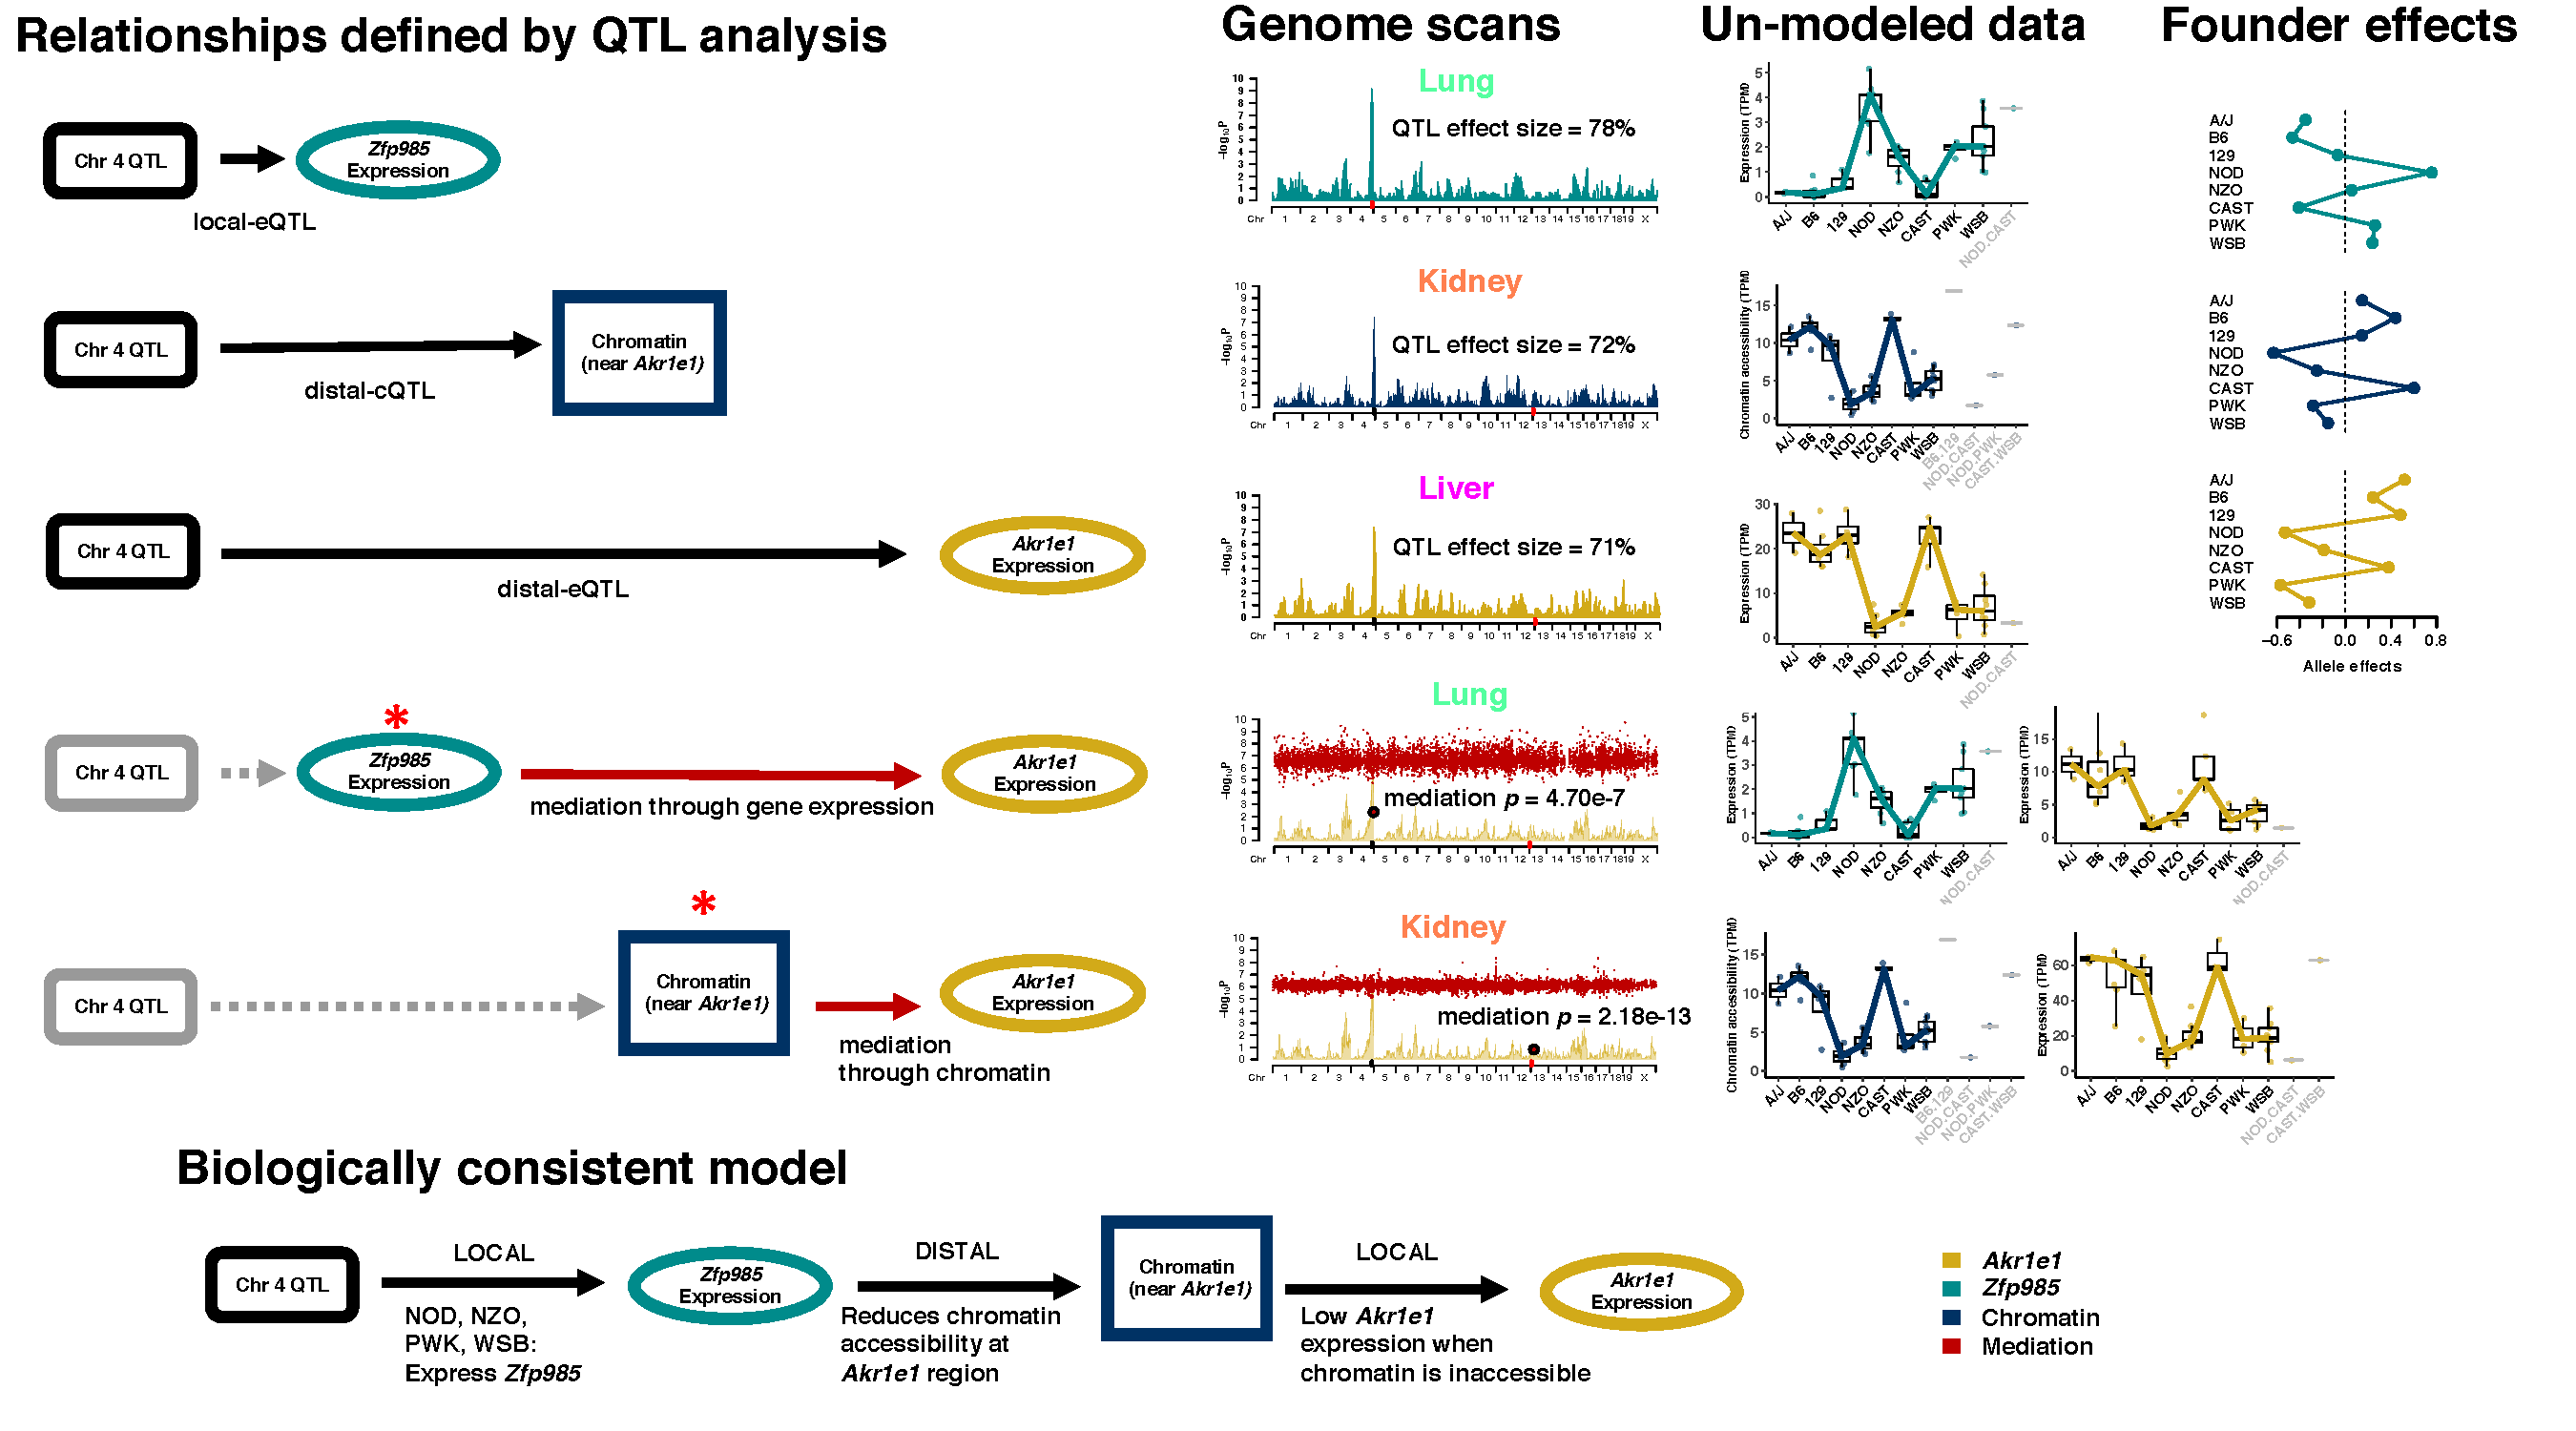
\includegraphics[width=\textwidth, trim={0in 0.1in 0in 0in}, clip]{figs/akr1e1_full_model.pdf}
\caption{\textbf{Complete mediation model for \textit{Akr1e1} distal-eQTL.} \label{fig:akr1e1_full_model.pdf}}
\end{figure*}

\begin{figure*}[hp]
\renewcommand{\familydefault}{\sfdefault}\normalfont
\centering
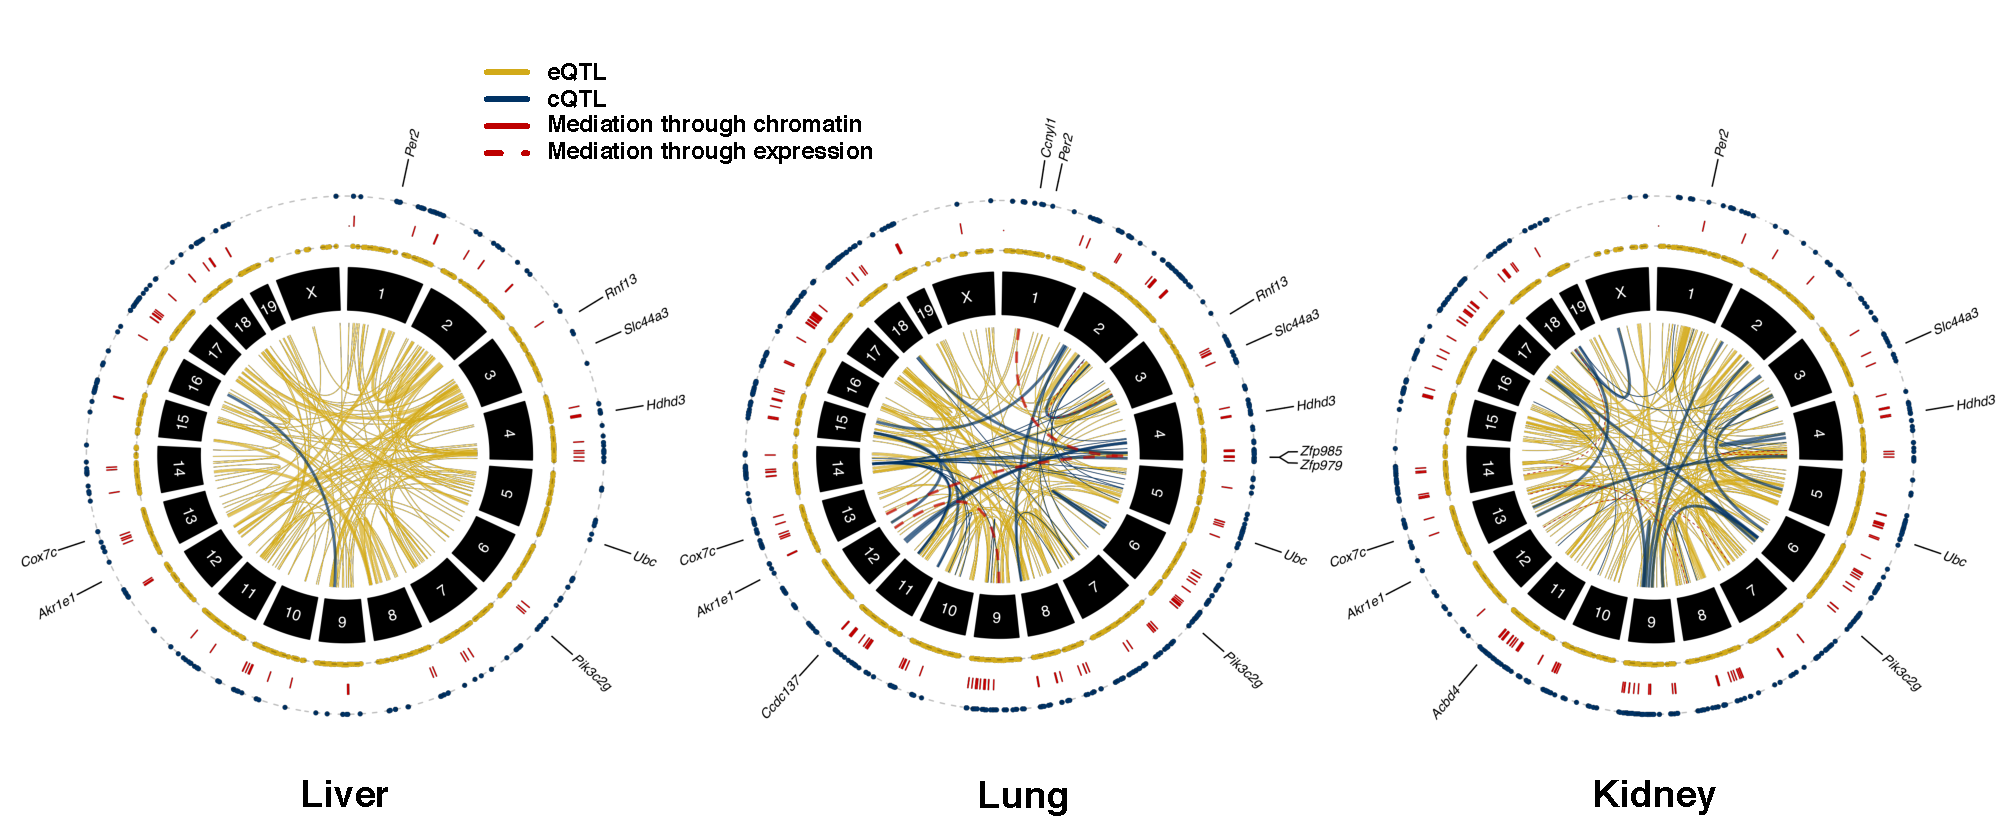
\includegraphics[width=\textwidth, trim={0.5in 0in 0.5in 0in}, clip]{figs/circos_over_tissues.pdf}
\caption{\textbf{Summaries of eQTL, cQTL, and mediation analyses.} Circos plots of eQTL (yellow), cQTL (blue), and mediation (red) in lung, liver, and kidney. The two outer rings of dots represent local-eQTL and local-cQTL detected by Method 3 at chromosome-wide significance, with red lines between connecting genes and chromatin sites for which chromatin mediation was detected. The inner circle contains connections representing distal-eQTL, distal-cQTL, and gene-gene mediation from Method 1. Thick lines represent QTL and mediators with permutation-based p-value (permP) $< 1 \times 10^{-6}$. The detected signals are primarily local, which also tend to be stronger than the observed distal signals. Fewer QTL and mediators are detected in liver tissue. Chromosome 17 seems to have most concentrated chromatin mediation signal across the three tissues.
\label{fig:circos_plot}}
\end{figure*}

